\documentclass[a4paper,12pt]{article}
\setlength{\headheight}{68.803pt}
\addtolength{\topmargin}{-56.803pt}

\usepackage[utf8]{inputenc}
\usepackage[T1]{fontenc}
\usepackage{lmodern}
\usepackage[nopatch=footnote]{microtype}
\usepackage{fvextra}
\DefineVerbatimEnvironment{Verbatim}{Verbatim}{
  breaklines=true,
  breakanywhere=true,
  frame=single,
  fontsize=\small
}

% Impostazione dei margini con geometry
\usepackage[
  left=1in,
  right=1in,
  top=3cm,
  bottom=1in
]{geometry}

\usepackage[
    colorlinks=true,
    linkcolor=black,
    urlcolor=blue,
    citecolor=blue,
    pdfborder={0 0 0},
    pdfauthor={Massimo Mantineo},
    pdftitle={Federated Learning con Ray.io e PyTorch},
    pdfsubject={Laboratorio di Reti e Sistemi Distribuiti: HANDS-ON 19},
]{hyperref}

\usepackage{graphicx}
\graphicspath{{../../assets/}{../../assets/ho1/}{../../assets/ho2/}{../../assets/ho3/}{../../assets/ho4/}{../../assets/ho5/}{../../assets/ho6/}{../../assets/ho7/}{../../assets/ho8/}{../../assets/ho10/}}
\usepackage{tikz}
\usetikzlibrary{positioning, arrows.meta, shapes.geometric}
\usepackage{listings}
\usepackage{xcolor}
\usepackage{amsmath, amssymb}
\usepackage{fancyhdr}
\usepackage{setspace}
\usepackage{pgfplots}
\pgfplotsset{compat=1.17}
\usepackage{booktabs}
\usepackage[skins, listings]{tcolorbox}
\usepackage{float}

\newtcblisting{terminal}[1][]{
    listing only,
    colback=black!85!white,
    colframe=black!70!white,
    colupper=green!80!white,
    coltitle=white,
    title=#1,
    fonttitle=\bfseries\sffamily,
    listing options={
        language={},
        basicstyle=\ttfamily\small\color{green!80!white},
        backgroundcolor={},
        frame=none,
        breaklines=true,
        showstringspaces=false,
        numbers=none
    },
    enhanced,
    drop shadow,
    arc=3mm
}

\newtcblisting{ccode}[1][]{
    listing only,
    colback=blue!3!white,
    colframe=blue!70!black,
    title=#1,
    fonttitle=\bfseries\sffamily,
    listing options={
        style=cstyle,
        backgroundcolor={},
        frame=none
    },
    enhanced,
    drop shadow,
    arc=3mm
}

\setlength{\footskip}{50pt}

\lstdefinestyle{cstyle}{
    language=C,
    basicstyle=\ttfamily\small,
    numbers=left,
    numberstyle=\tiny,
    stepnumber=1,
    numbersep=5pt,
    backgroundcolor=\color{white},
    showspaces=false,
    showstringspaces=false,
    showtabs=false,
    frame=single,
    tabsize=4,
    captionpos=b,
    breaklines=true,
    breakatwhitespace=true,
    keywordstyle=\color{blue}\bfseries,
    commentstyle=\color{green!50!black},
    stringstyle=\color{red},
}
\lstset{style=cstyle}

% Impostazione di fancyhdr per header e footer
\pagestyle{fancy}
\fancyhf{}

\fancyhead[L]{%
  \parbox[b]{0.45\textwidth}{%
    \small
    Student Name: Massimo Mantineo\\
    Student ID: 541924
    \vspace{20pt}
  }%
}
\fancyhead[C]{%
  \parbox[b]{0.2\textwidth}{%
    \centering
    \normalsize \bfseries
    LabReSiD25\\
    Hands-On 19
    \vspace{20pt}
  }%
}
\fancyhead[R]{%
  \parbox[b]{0.35\textwidth}{%
    \flushright
    \includegraphics[width=3.5cm]{\detokenize{logo_unime_orizontale.png}}
    \vspace{15pt}
  }%
}

\renewcommand{\contentsname}{Indice}

\title{\vspace{-2cm}Report: Federated Learning con Ray.io e PyTorch\\
\large (Hands-On 19)}
\author{Massimo Mantineo \\ Matricola: 541924}
\date{MESSINA, A.A. 2024/2025}

\begin{document}

% Pagina di copertina
\begin{titlepage}
    \thispagestyle{empty}
    \centering
    \vspace*{1cm}
    \includegraphics[width=6cm]{\detokenize{logo_unime_orizontale.png}}\par\vspace{1cm}
    \vspace{2cm}
    {\Large \textbf{Università degli Studi di Messina}\par}
    {\large Dipartimento MIFT - Corso di Laurea Triennale in Informatica (L-31)\par}
    \vspace*{1cm}
    {\large Laboratorio di Reti e Sistemi Distribuiti\par}
    \vspace{1cm}
    {\Large \textbf{HANDS-ON 19:}\\
    Federated Learning con Ray.io e PyTorch\par}
    \vspace{2cm}
    {\large Massimo Mantineo \par}
    {\large Matricola: 541924 \par}
    \vfill
    {\large Messina, A.A. 2024/2025 \par}
\end{titlepage}

\clearpage
\pagestyle{fancy}
\tableofcontents
\newpage

\section{Problem Statement}
L'obiettivo di questo Hands-On è l'implementazione di un sistema di \textbf{Federated Learning (FL)} per la classificazione di immagini del dataset MNIST. A differenza del paradigma tradizionale centralizzato, il Federated Learning permette di addestrare modelli di Machine Learning su dati distribuiti, mantenendo la privacy dei dati locali. 

In questo esperimento, abbiamo utilizzato \textbf{Ray.io} come framework di orchestrazione distribuita e \textbf{PyTorch} per la definizione e l'addestramento del modello neurale.

\section{Stato dell'Arte}
Il Federated Learning si basa sul concetto di portare il calcolo dai dati, invece dei dati al calcolo.

\begin{figure}[H]
    \centering
    \begin{tikzpicture}[
        node distance=1.5cm,
        aggregator/.style={rectangle, draw=blue!70, fill=blue!5, thick, minimum width=3.5cm, minimum height=1.2cm, align=center, font=\bfseries\sffamily},
        worker/.style={circle, draw=green!70, fill=green!5, thick, minimum size=1.5cm, align=center, font=\tiny\sffamily},
        arrow/.style={-Stealth, thick, gray!80}
    ]
        % Aggregator
        \node[aggregator] (agg) {GLOBAL AGGREGATOR\\(Global Model $W$)};

        % Workers
        \node[worker, below left=2cm and 1cm of agg] (w1) {Worker 1\\(Local Data $D\_1$)};
        \node[worker, below=2.5cm of agg] (w2) {Worker 2\\(Local Data $D\_2$)};
        \node[worker, below right=2cm and 1cm of agg] (w3) {Worker 3\\(Local Data $D\_3$)};

        % Downlink
        \draw[arrow, blue!70] (agg.south) -- node[left, font=\tiny, color=black] {Broadcast Weights} (w1.north);
        \draw[arrow, blue!70] (agg.south) -- (w2.north);
        \draw[arrow, blue!70] (agg.south) -- node[right, font=\tiny, color=black] {Model Sync} (w3.north);

        % Uplink
        \draw[arrow, green!70!black, dashed] (w1.east) to[bend left=20] node[below, font=\tiny, sloped, color=black] {Local Gradients $\nabla W\_1$} (agg.west);
        \draw[arrow, green!70!black, dashed] (w2.north west) to[bend left=10] (agg.south west);
        \draw[arrow, green!70!black, dashed] (w3.west) to[bend right=20] (agg.east);
        
        \node[below=0.5cm of w2, font=\itshape\small] {Decentralized Training (Privacy Preserved)};
    \end{tikzpicture}
    \caption{Ciclo di addestramento nel Federated Learning: Distribuzione pesi e Aggregazione gradienti.}
    \label{fig:fl\_workflow}
\end{figure}

Il processo tipico prevede:
\begin{enumerate}
    \item Un'entità centrale (\textbf{Aggregator}) che invia i pesi del modelo globale ai partecipanti.
    \item I partecipanti (\textbf{Workers}) che addestrano localmente il modello sui propri dati.
    \item L'invio degli aggiornamenti (gradienti o pesi) all'Aggregator.
    \item L'aggregazione degli aggiornamenti tramite algoritmi come il \textbf{Federated Averaging (FedAvg)}.
\end{enumerate}

L'algoritmo FedAvg calcola la media pesata dei parametri del modello:
\begin{equation}
    w\_{t+1} = \sum\_{k=1}^{K} \frac{n\_k}{n} w\_{t+1}^k
\end{equation}
dove $n\_k$ è il numero di esempi del worker $k$ e $n$ il totale degli esempi.

\section{Metodologia ed Implementazione}
Il sistema è stato implementato con 1 Aggregator e 6 Worker distribuiti come \textbf{Ray Actors}.

\subsection{Partizionamento dei Dati}
Le 60.000 immagini del set di training di MNIST sono state suddivise in modo casuale (\textbf{IID split}) tra i 6 worker, assegnando 10.000 immagini a ciascuno. Ogni worker gestisce il proprio \texttt{DataLoader} locale.

\subsection{Architettura Distribuita}
\begin{itemize}
    \item \textbf{FederatedWorker}: Riceve i pesi globali, esegue 1 epoca di training locale e restituisce i pesi aggiornati.
    \item \textbf{FederatedAggregator}: Coordina i round di comunicazione, esegue l'aggregazione FedAvg e valuta il modello globale su un set di test centrale (10.000 immagini).
\end{itemize}


\subsection{Istruzioni di Esecuzione}
L'addestramento federato viene gestito tramite Makefile:
\begin{terminal}[Run]
$ make install # Setup ambiente
$ make run     # Avvio training federato
\end{terminal}

\section{Risultati}
Il sistema è stato testato per 3 round di comunicazione. I log mostrano un rapido incremento dell'accuratezza globale:

\begin{terminal}[Log Addestramento Federato]
>>> Initializing Federated Learning with 6 workers...
>>> Round 1 starting...
Round 1 - Global Test Accuracy: 92.48%
>>> Round 2 starting...
Round 2 - Global Test Accuracy: 95.21%
>>> Round 3 starting...
Round 3 - Global Test Accuracy: 96.16%
Training finished.
\end{terminal}

L'accuratezza finale del \textbf{96.16\%} ottenuta in soli 3 round dimostra l'efficacia dell'approccio federato nella convergenza del modello MLP.

\section{Conclusioni e Sviluppi Futuri}
L'implementazione ha dimostrato come Ray.io semplifichi drasticamente la gestione di attori distribuiti per compiti di intelligenza artificiale. Il Federated Learning si è rivelato un metodo robusto per l'addestramento distribuito, riuscendo a mantenere prestazioni paragonabili alla versione centralizzata pur mantenendo i dati frammentati su worker indipendenti.

\end{document}
